\documentclass{article}

\usepackage{fancyhdr} % Required for custom headers
\usepackage{lastpage} % Required to determine the last page for the footer
\usepackage{extramarks} % Required for headers and footers
\usepackage[usenames,dvipsnames]{color} % Required for custom colors
\usepackage{graphicx} % Required to insert images
\usepackage{listings} % Required for insertion of code
\usepackage{courier} % Required for the courier font
\usepackage{lipsum} % Used for inserting dummy 'Lorem ipsum' text into the template
\usepackage{amsmath}
\usepackage{amssymb}
\usepackage{mathtools, xparse}
\usepackage{booktabs}
\usepackage{bigstrut}
\usepackage{float}
\usepackage{hyperref}
\usepackage{color}
\usepackage{algorithm}
\usepackage{caption}
\captionsetup{skip=0pt}
\usepackage{algpseudocode}
\usepackage{multirow}
\usepackage{subfigure}
\usepackage{longtable}
\usepackage{supertabular}

\DeclarePairedDelimiter{\norm}{\lVert}{\rVert}
\DeclarePairedDelimiter\abs{\lvert}{\rvert}%

\hypersetup{
    colorlinks   = true,    % Colours links instead of ugly boxes
    urlcolor     = red,    % Colour for external hyperlinks
    linkcolor    = red,    % Colour of internal links
    citecolor    = red      % Colour of citations
}
% Margins
\topmargin=-0.45in
\evensidemargin=0in
\oddsidemargin=0in
\textwidth=6.5in
\textheight=9.0in
\headsep=0.25in

\linespread{1.1} % Line spacing

% Set up the header and footer
\pagestyle{fancy}
\lhead{\hmwkAuthorName} % Top left header
\rhead{\hmwkClass\ : \hmwkID} % Top center head
%\rhead{\firstxmark} % Top right header
\lfoot{\lastxmark} % Bottom left footer
\cfoot{} % Bottom center footer
\rfoot{Page\ \thepage\ of\ \protect\pageref*{LastPage}} % Bottom right footer
\renewcommand\headrulewidth{0.4pt} % Size of the header rule
\renewcommand\footrulewidth{0.4pt} % Size of the footer rule
\renewcommand{\subsectionmark}[1]{\markboth{#1}{}}
\setlength\parindent{0pt} % Removes all indentation from paragraphs

%----------------------------------------------------------------------------------------
%	CODE INCLUSION CONFIGURATION
%----------------------------------------------------------------------------------------

\definecolor{MyDarkGreen}{rgb}{0.0,0.4,0.0} % This is the color used for comments
\lstloadlanguages{Perl} % Load Perl syntax for listings, for a list of other languages supported see: ftp://ftp.tex.ac.uk/tex-archive/macros/latex/contrib/listings/listings.pdf
\lstset{language=Perl, % Use Perl in this example
    frame=single, % Single frame around code
    basicstyle=\small\ttfamily, % Use small true type font
    keywordstyle=[1]\color{Blue}\bf, % Perl functions bold and blue
    keywordstyle=[2]\color{Purple}, % Perl function arguments purple
    keywordstyle=[3]\color{Blue}\underbar, % Custom functions underlined and blue
    identifierstyle=, % Nothing special about identifiers                                         
    commentstyle=\usefont{T1}{pcr}{m}{sl}\color{MyDarkGreen}\small, % Comments small dark green courier font
    stringstyle=\color{Purple}, % Strings are purple
    showstringspaces=false, % Don't put marks in string spaces
    tabsize=5, % 5 spaces per tab
    %
    % Put standard Perl functions not included in the default language here
    morekeywords={rand},
    %
    % Put Perl function parameters here
    morekeywords=[2]{on, off, interp},
    %
    % Put user defined functions here
    morekeywords=[3]{test},
    %
    morecomment=[l][\color{Blue}]{...}, % Line continuation (...) like blue comment
    numbers=left, % Line numbers on left
    firstnumber=1, % Line numbers start with line 1
    numberstyle=\tiny\color{Blue}, % Line numbers are blue and small
    stepnumber=5 % Line numbers go in steps of 5
}

% Creates a new command to include a perl script, the first parameter is the filename of the script (without .pl), the second parameter is the caption
\newcommand{\perlscript}[2]{
    \begin{itemize}
        \item[]\lstinputlisting[caption=#2,label=#1]{#1.py}
    \end{itemize}
}
\newcommand{\cppscript}[1]{
    \begin{itemize}
        \item[]\lstinputlisting[]{#1}
    \end{itemize}
}

%----------------------------------------------------------------------------------------
%	DOCUMENT STRUCTURE COMMANDS
%	Skip this unless you know what you're doing
%----------------------------------------------------------------------------------------

% Header and footer for when a page split occurs within a problem environment
\newcommand{\enterProblemHeader}[1]{
    \nobreak\extramarks{#1}{#1 continued on next page\ldots}\nobreak
    \nobreak\extramarks{#1 (continued)}{#1 continued on next page\ldots}\nobreak
}

% Header and footer for when a page split occurs between problem environments
\newcommand{\exitProblemHeader}[1]{
    \nobreak\extramarks{#1 (continued)}{#1 continued on next page\ldots}\nobreak
    \nobreak\extramarks{#1}{}\nobreak
}

%\setcounter{secnumdepth}{0} % Removes default section numbers
\newcounter{homeworkProblemCounter} % Creates a counter to keep track of the number of problems

\newcommand{\homeworkProblemName}{}
\newenvironment{homeworkProblem}[1][Problem \arabic{homeworkProblemCounter}]{ % Makes a new environment called homeworkProblem which takes 1 argument (custom name) but the default is "Problem #"
    \stepcounter{homeworkProblemCounter} % Increase counter for number of problems
    \renewcommand{\homeworkProblemName}{#1} % Assign \homeworkProblemName the name of the problem
    \section{\homeworkProblemName} % Make a section in the document with the custom problem count
    \enterProblemHeader{\homeworkProblemName} % Header and footer within the environment
    }{
    \exitProblemHeader{\homeworkProblemName} % Header and footer after the environment
}

\newcommand{\problemAnswer}[1]{ % Defines the problem answer command with the content as the only argument
\noindent\framebox[\columnwidth][c]{\begin{minipage}{0.98\columnwidth}#1\end{minipage}} % Makes the box around the problem answer and puts the content inside
}

\newcommand{\homeworkSectionName}{}
\newenvironment{homeworkSection}[1]{ % New environment for sections within homework problems, takes 1 argument - the name of the section
    \renewcommand{\homeworkSectionName}{#1} % Assign \homeworkSectionName to the name of the section from the environment argument
    \subsection{\homeworkSectionName} % Make a subsection with the custom name of the subsection
    \enterProblemHeader{\homeworkProblemName\ [\homeworkSectionName]} % Header and footer within the environment
    }{
    \enterProblemHeader{\homeworkProblemName} % Header and footer after the environment
}

%----------------------------------------------------------------------------------------
%	NAME AND CLASS SECTION
%----------------------------------------------------------------------------------------

\newcommand{\hmwkID}{hw01} % Assignment title
\newcommand{\hmwkTitle}{Displacement and Strain}
\newcommand{\hmwkDueDate}{Thursday,\ Nov\ 2,\ 2017} % Due date
\newcommand{\hmwkClass}{Principles of Biomedical Ultrasound and Photoacoustics} % Course/class
\newcommand{\hmwkClassTime}{10:30am} % Class/lecture time
\newcommand{\hmwkClassInstructor}{Jones} % Teacher/lecturer
\newcommand{\hmwkAuthorName}{106061531 Fu-En Wang} % Your name

%----------------------------------------------------------------------------------------
%	TITLE PAGE
%----------------------------------------------------------------------------------------

\title{
    \vspace{2in}
    \textmd{\textbf{\hmwkClass}}\\
    \textmd{\textbf{\hmwkID: \hmwkTitle}} \\
    \normalsize\vspace{0.1in}\small{Due\ on\ \hmwkDueDate}\\
    \vspace{3in}
}

\author{\textbf{\hmwkAuthorName}}
\date{} % Insert date here if you want it to appear below your name

%----------------------------------------------------------------------------------------

\begin{document}
\maketitle
\newpage

\section{Introduction}
For \textbf{Focused Ultrasound Thermal Therapy}, an important technique is to estimate the temperature change before and after applying it.
The estimation can be derived by the echo-time shift before and after heating. Moreover, the temperature change can be formula as:
\begin{align}
\Delta T(z) = \frac{C_0}{2} \cdot K \cdot \frac{\partial \Delta t(z)}{\partial z}
\label{eq:temp change}
\end{align}
where $\Delta T(z)$ is the temperature change, $C_0$ is the speed of sound, $K$ is a constant, $\frac{\partial \Delta t(z)}{\partial z}$
is the \textbf{thermal strain}.

In this homework, we need to finish the following requirements:
\begin{enumerate}
	\item Estimate echo time shift in $\mu s$ as a function of depth
	\item Estimate thermal strain in \% as a function of depth
\end{enumerate}

\section{Source Code}
In this zip archive, there are two matlab source code files:
\begin{enumerate}
	\item \textbf{EE6265\_HW1\_106061531.m}
	\item \textbf{Windows.m}
\end{enumerate}
"EE6265\_HW1\_106061531.m" is the main flow of this homework. It will use the class \textbf{Windows} in "Windows.m" to create
an object, which can manage each window and makes our code more elegant, and plot figures with our given parameters.

\section{Problems}
In Equation \ref{eq:temp change}, the term $\Delta t(z)$ is the echo-time shift before and after ultrasound heating. Because 
$\Delta t(z)$ is a function of $z$, which means $\Delta t(z)$ will vary at different depth. As a result, we can divide the 
pre-signal and post-signal into several frames with certain window size and apply cross-correlation for each pre/post window
pair. By this way, we can estimate the time shift for each window. For more accurate result, we can upsample the origin signal
to get more sample points and higher sample rate. In this homework, I upsample the signal to triple origin sample rate
($3 \times f_s$) and use a moving average filter with size 5 to denoise the echo-time shift.

In the following section, I will show and explain several results.
\subsection{Echo-Time Shift}
In this part, I run experiments with different paramters. Windows size is 2, 6, 10 wavelength, and each combines with different 
overlap ratio (0, 0.5, 0.75). Figure [\ref{fig:shift-2}, \ref{fig:shift-6}, \ref{fig:shift-10}] show the Echo-Time Shift
as a function of $z$ for M = 2, 6 and 10, respectively.

In Figure \ref{fig:shift-2}, we can find that the echo-time shift is very unstable. Because the window size is only 2
wavelength, the small window will be very sensitive to noise. However, it will also preserve more detailed information of
our signal. Also, same for the overlap ratio. When the ratio is small, the detailed information of signal will be harder
to captured, while larger ratio can extract the variation of signal, so the change of echo-time shift will be more obvious.

\begin{figure}[H]
    \centering
    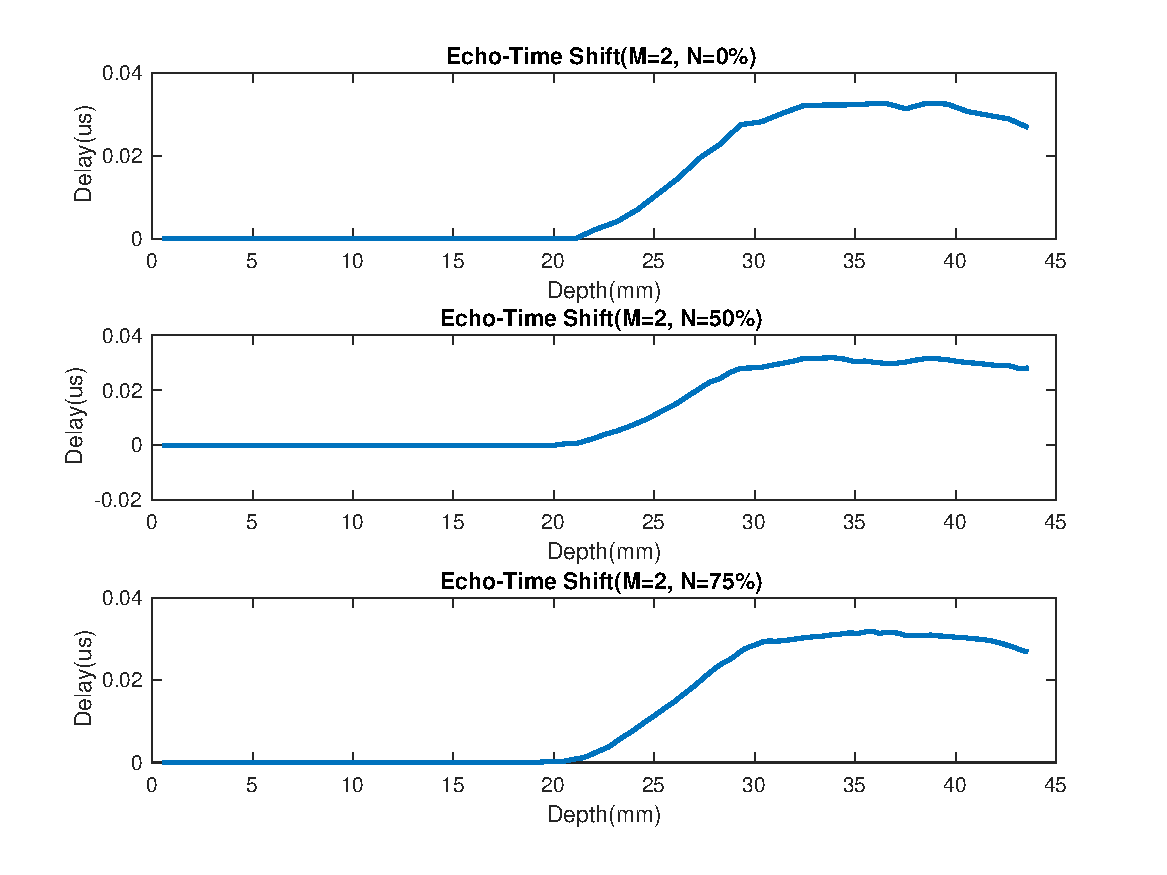
\includegraphics[width=0.82\textwidth]{src/shift_2.pdf}
    \caption{Echo-Time Shift (M=2)}
    \label{fig:shift-2}
\end{figure}
\begin{figure}[H]
    \centering
    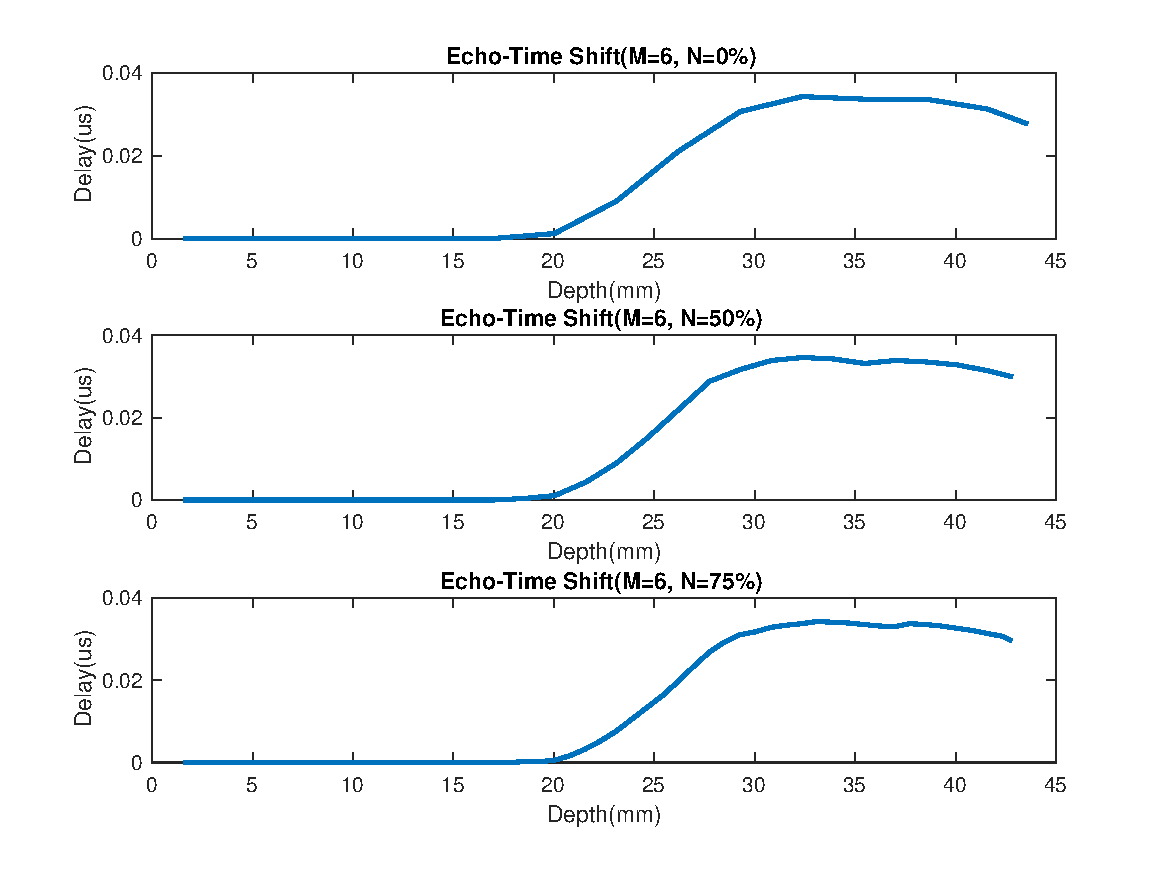
\includegraphics[width=0.82\textwidth]{src/shift_6.pdf}
    \caption{Echo-Time Shift (M=6)}
    \label{fig:shift-6}
\end{figure}
\begin{figure}[H]
    \centering
    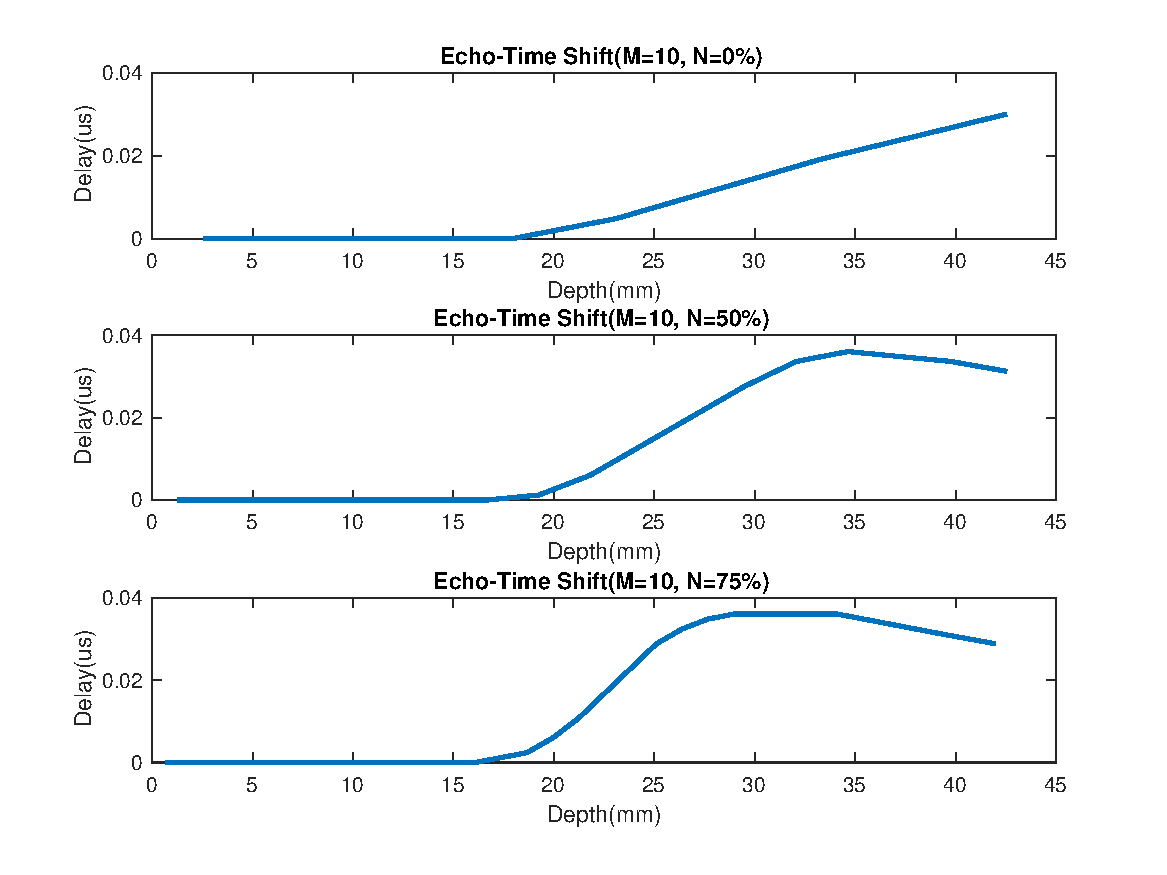
\includegraphics[width=0.82\textwidth]{src/shift_10.pdf}
    \caption{Echo-Time Shift (M=10)}
    \label{fig:shift-10}
\end{figure}

In Figure \ref{fig:shift-6}, the result becomes much more smoothed than Figure \ref{fig:shift-2}. Because we have a larger 
window size, it will be more robust for noise but also loss more detailed information. Similar to Figure \ref{fig:shift-2}, 
the result gets more smoothed when applying larger overlap ratio.

In Figure \ref{fig:shift-10}, we get a more smoothed result than Figure \ref{fig:shift-6} because the window size is larger too.
However, I think 10 wavelength window size is not a suitable number for such task because the result is \textbf{too smoothed},
which losses too much information of signal and we cannot analyze it. As a result, I think 6 wavelength window size is the best 
choice for this task in homework.

From the result of Figure [\ref{fig:shift-2}, \ref{fig:shift-6}, \ref{fig:shift-10}], we can find that larger window size and
smaller overlap ratio will give a more smoothed result, while smaller window size and larger overlap ratio will preserve 
more detailed information but sensitive to noise.

\end{document}















